

\subsection{Planning and Execution}

We reuse the learned stage-wise constraint model in an optimization-based planner. For this experiment, the state $x_t\in\mathcal{X}$ is the end-effector pose expressed in a frozen bar-fixed frame $\mathcal{B}$, i.e., $x_t=(p_t^{\mathcal{B}},R_t^{\mathcal{B}})$, where $p_t^{\mathcal{B}}\in\mathbb{R}^3$ and $R_t^{\mathcal{B}}\in SO(3)$ denote position and orientation relative to the bar. The start state, goal state, subgoals, and all task features are represented in the same frame.

Let $(\widehat{\Gamma},\widehat{\mathcal{P}})$ be the constraint model recovered from the demonstrations, with learned modes $\widehat{\gamma}_{k,j}$ and parameters $\widehat{\eta}_{k,j}$.

For each intermediate stage, the subgoal $g_k$ is set to the average of the corresponding stage endpoints over all demonstrations. The final subgoal is the desired terminal state, $g_K=x_{\mathrm{goal}}$.

To use the learned equality and inequality constraints in a common objective, we define the violation residual
\begin{equation}
r_{k,j}(x)=
\begin{cases}
0, & \widehat{\gamma}_{k,j}=\varnothing,\\
\phi_j(x)-\widehat{\eta}_{k,j}, & \widehat{\gamma}_{k,j}=\mathrm{eq},\\
\left[\widehat{\eta}_{k,j}-\phi_j(x)\right]_+, & \widehat{\gamma}_{k,j}=\mathrm{lb},\\
\left[\phi_j(x)-\widehat{\eta}_{k,j}\right]_+, & \widehat{\gamma}_{k,j}=\mathrm{ub},
\end{cases}
\label{eq:barclear_constraint_residual}
\end{equation}
where $[z]_+=\max(z,0)$. Thus, an equality constraint is penalized according to its deviation from the learned target, while an inequality constraint incurs a penalty only on its infeasible side.

The planner discretizes each stage segment according to a fixed spatial waypoint spacing. If stage $k$ contains $T_k$ waypoints, its boundary is $b_k=1+\sum_{l=1}^{k}T_l$, which defines the waypoint schedule $B=\{b_k\}_{k=0}^{K}$. Thus, $B$ specifies only the waypoint allocation across stages and does not prescribe their execution durations. Planning is then formulated as
\begin{equation}
\begin{aligned}
\min_{\tau=\{x_t\}_{t=1}^{T}}\quad
& J_{\mathrm{smooth}}(\tau)
+\lambda_c\sum_{k=1}^{K}\sum_{t\in\mathcal{I}_k(B)}\sum_{j=1}^{F}r_{k,j}(x_t)^2 \\
\mathrm{s.t.}\quad
& x_1=x_{\mathrm{start}},\\
& x_{b_k-1}=g_k, \qquad k=1,\dots,K,\\
& \tau\in\mathcal{C}_{\mathrm{known}}.
\end{aligned}
\label{eq:barclear_trajectory_optimization}
\end{equation}
Here, $J_{\mathrm{smooth}}$ penalizes path length and rapid changes in end-effector position and orientation, and $\lambda_c$ balances trajectory regularity against satisfaction of the learned constraints. The stage intervals $\mathcal{I}_k(B)$ determine which row of $\widehat{\Gamma}$ is applied to each waypoint, while $\mathcal{C}_{\mathrm{known}}$ collects the known geometric and kinematic feasibility requirements. The optimization is therefore a nonlinear least-squares problem whose residuals combine trajectory regularization with violations of the learned stage-wise constraints.

The problem is solved numerically from multiple initial trajectories. After optimization, the task-space poses are transformed from the bar frame to the robot base frame and converted to joint-space waypoints using sequential inverse kinematics. Each IK problem is initialized with the solution of the preceding waypoint to keep the joint trajectory on a consistent solution branch. The joint path is then time-parameterized using nominal approach and task speeds, with local speed reduction around stage transitions and enforcement of the joint velocity and acceleration limits. The resulting joint positions, velocities, accelerations, and timestamps are sent to a standard ROS joint-position trajectory controller, which interpolates the desired motion and communicates position commands to the robot at $200\,\mathrm{Hz}$.

\subsection{Results}

We evaluate whether the learned constraints support successful task execution on the real robot. Because neither ground-truth stage cutpoints nor ground-truth constraints are available for this task, we assess performance using three task-level criteria: obstacle passing, sweeping the objects off the bar, and sweeping the objects off the table. We varied the positions and orientations of both the obstacle and the bar and evaluated 20 execution trials. The robot passed the obstacle in 18 of 20 trials ($90\%$); the two failures were caused by excessively tilted initial tool poses. It successfully swept the objects off the bar in all 20 trials ($100\%$) and swept the objects off the table in 17 of 20 trials ($85\%$). The latter failures occurred when too many objects were used or when the objects rolled readily on the table.

\begin{figure*}[t]
    \centering
    \subfloat[Stage 1: approach]{
        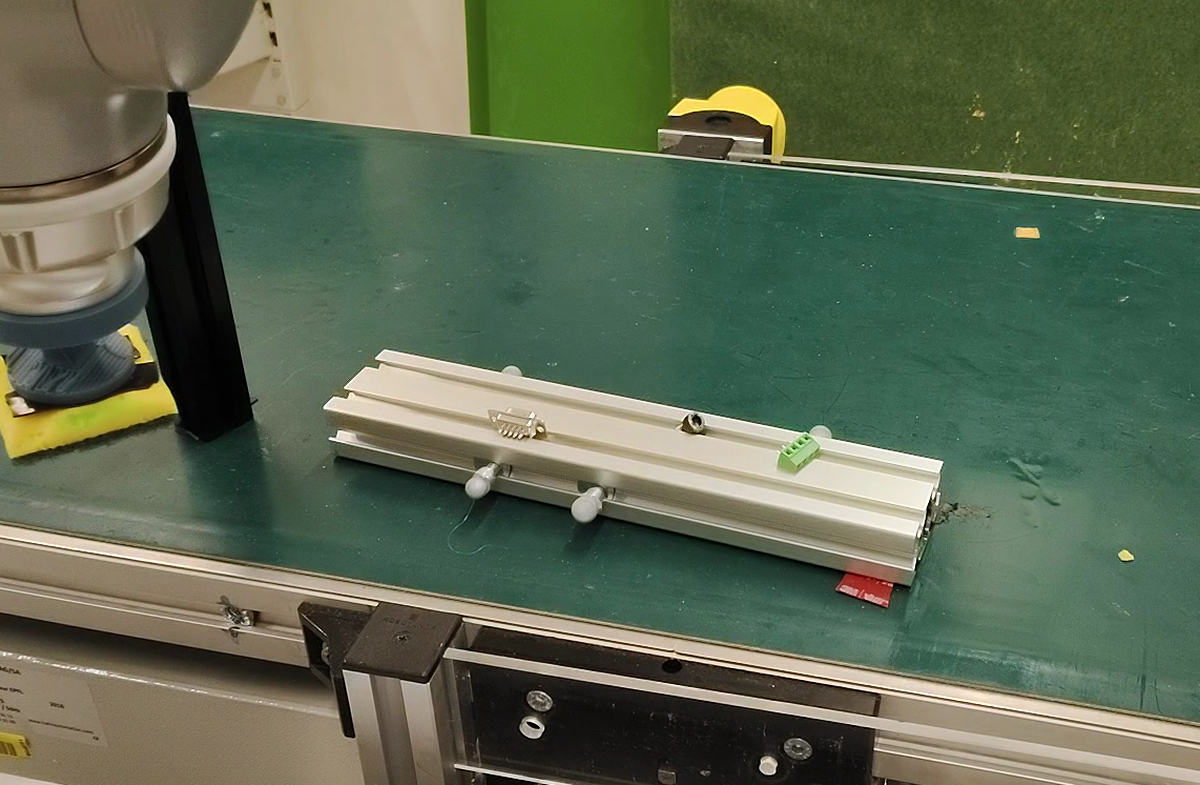
\includegraphics[width=0.242\textwidth]{figs/barclear_asss10_stage1.png}
    }\hfill
    \subfloat[Stage 2: bar sweeping]{
        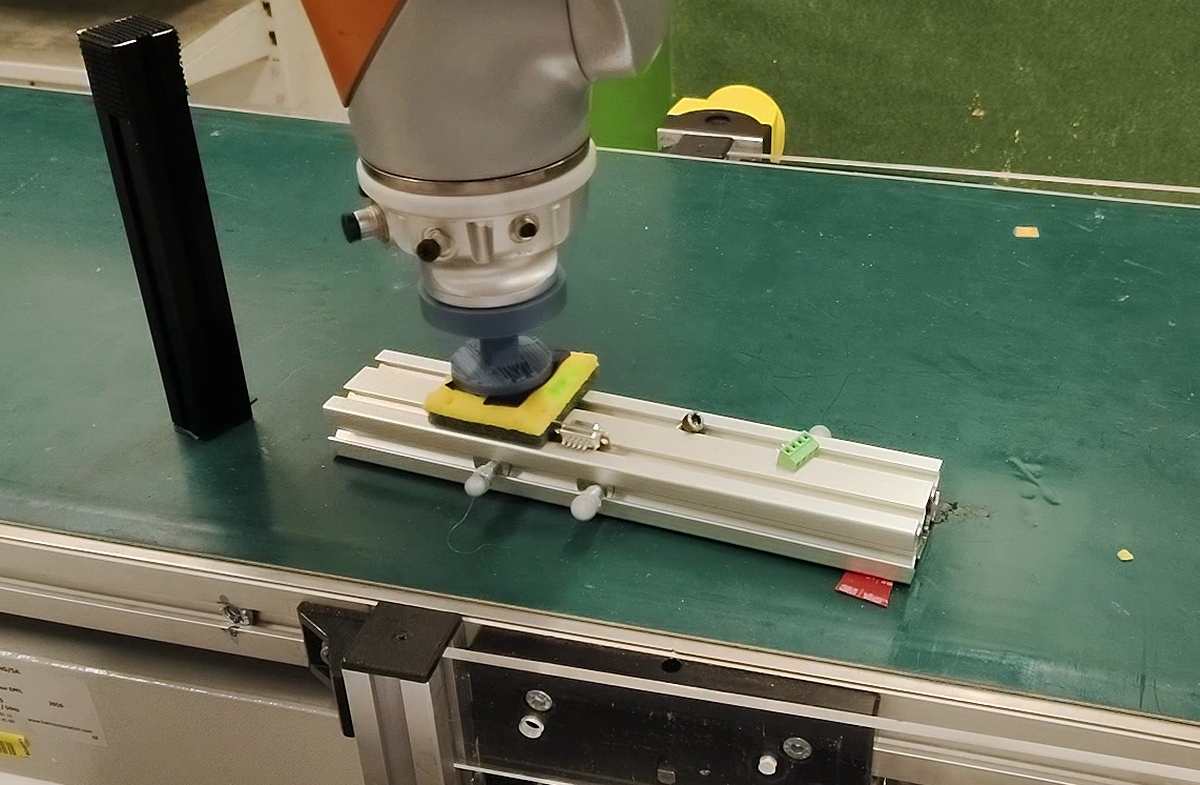
\includegraphics[width=0.242\textwidth]{figs/barclear_asss10_stage2.png}
    }\hfill
    \subfloat[Stage 3: repositioning]{
        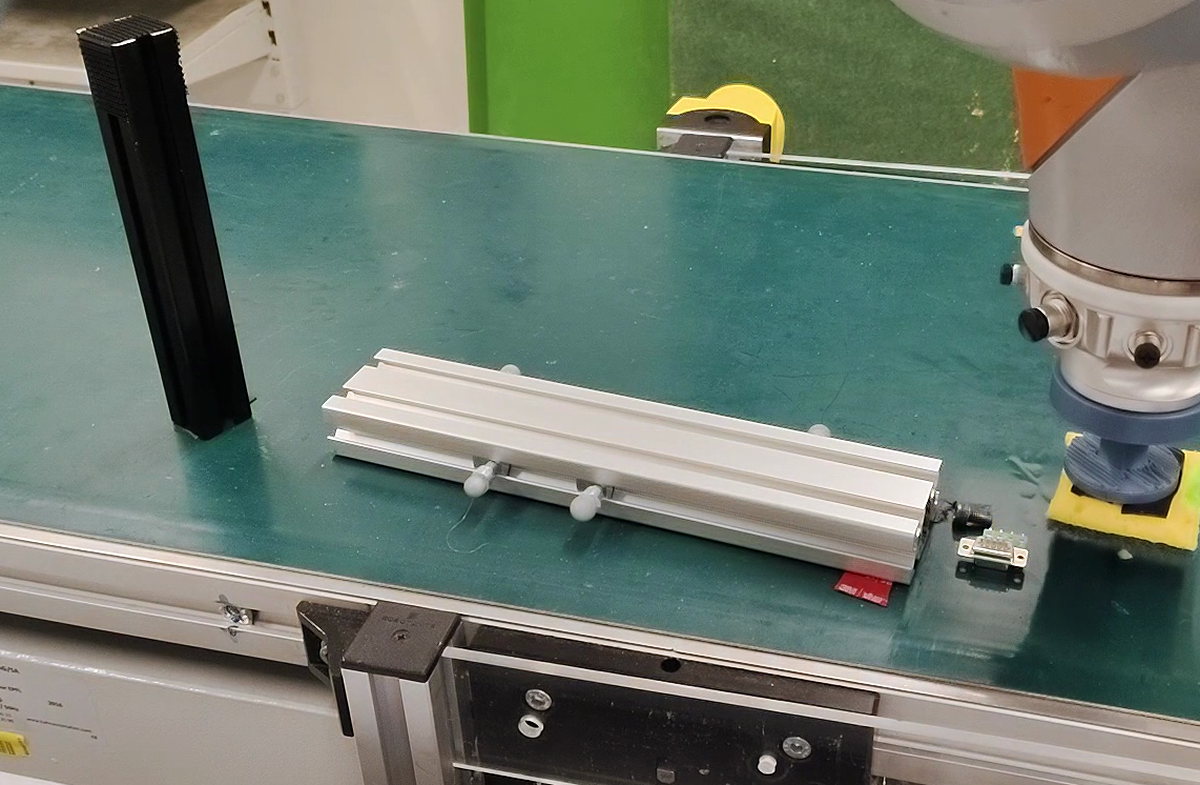
\includegraphics[width=0.242\textwidth]{figs/barclear_asss10_stage3.png}
    }\hfill
    \subfloat[Stage 4: table sweeping]{
        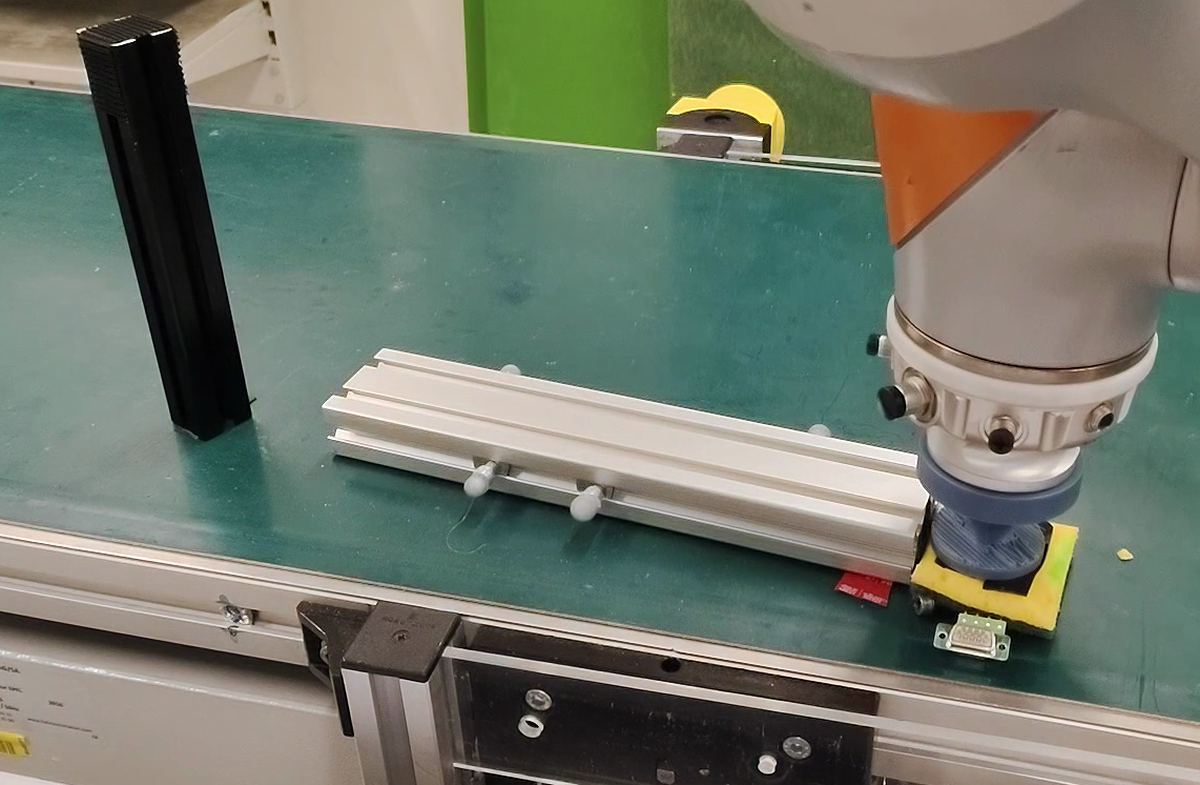
\includegraphics[width=0.242\textwidth]{figs/barclear_asss10_stage4.png}
    }
    \caption{Representative snapshots from a real-robot execution of the bar-clearing task using the learned stage-wise constraints. The four snapshots show the first four stages: (a) approaching the bar while passing the obstacle; (b) sweeping the litter objects from the bar onto the table; (c) repositioning the tool between the two sweeping motions; and (d) sweeping the litter objects off the table. The final retreat stage is omitted.}
    \label{fig:barclear_execution_snapshots}
\end{figure*}

The learned constraints can also be transferred to related environments. As shown in Fig.~\ref{fig:barclear_transfer}, we replace the straight bar with a curved bar and introduce an additional obstacle. The geometry of the curved bar is known and is used to compute the corresponding bar-relative features, while the learned stage-wise constraint model remains unchanged. The robot successfully completes the bar-clearing task in this transferred setting.

\begin{figure}[t]
    \centering
    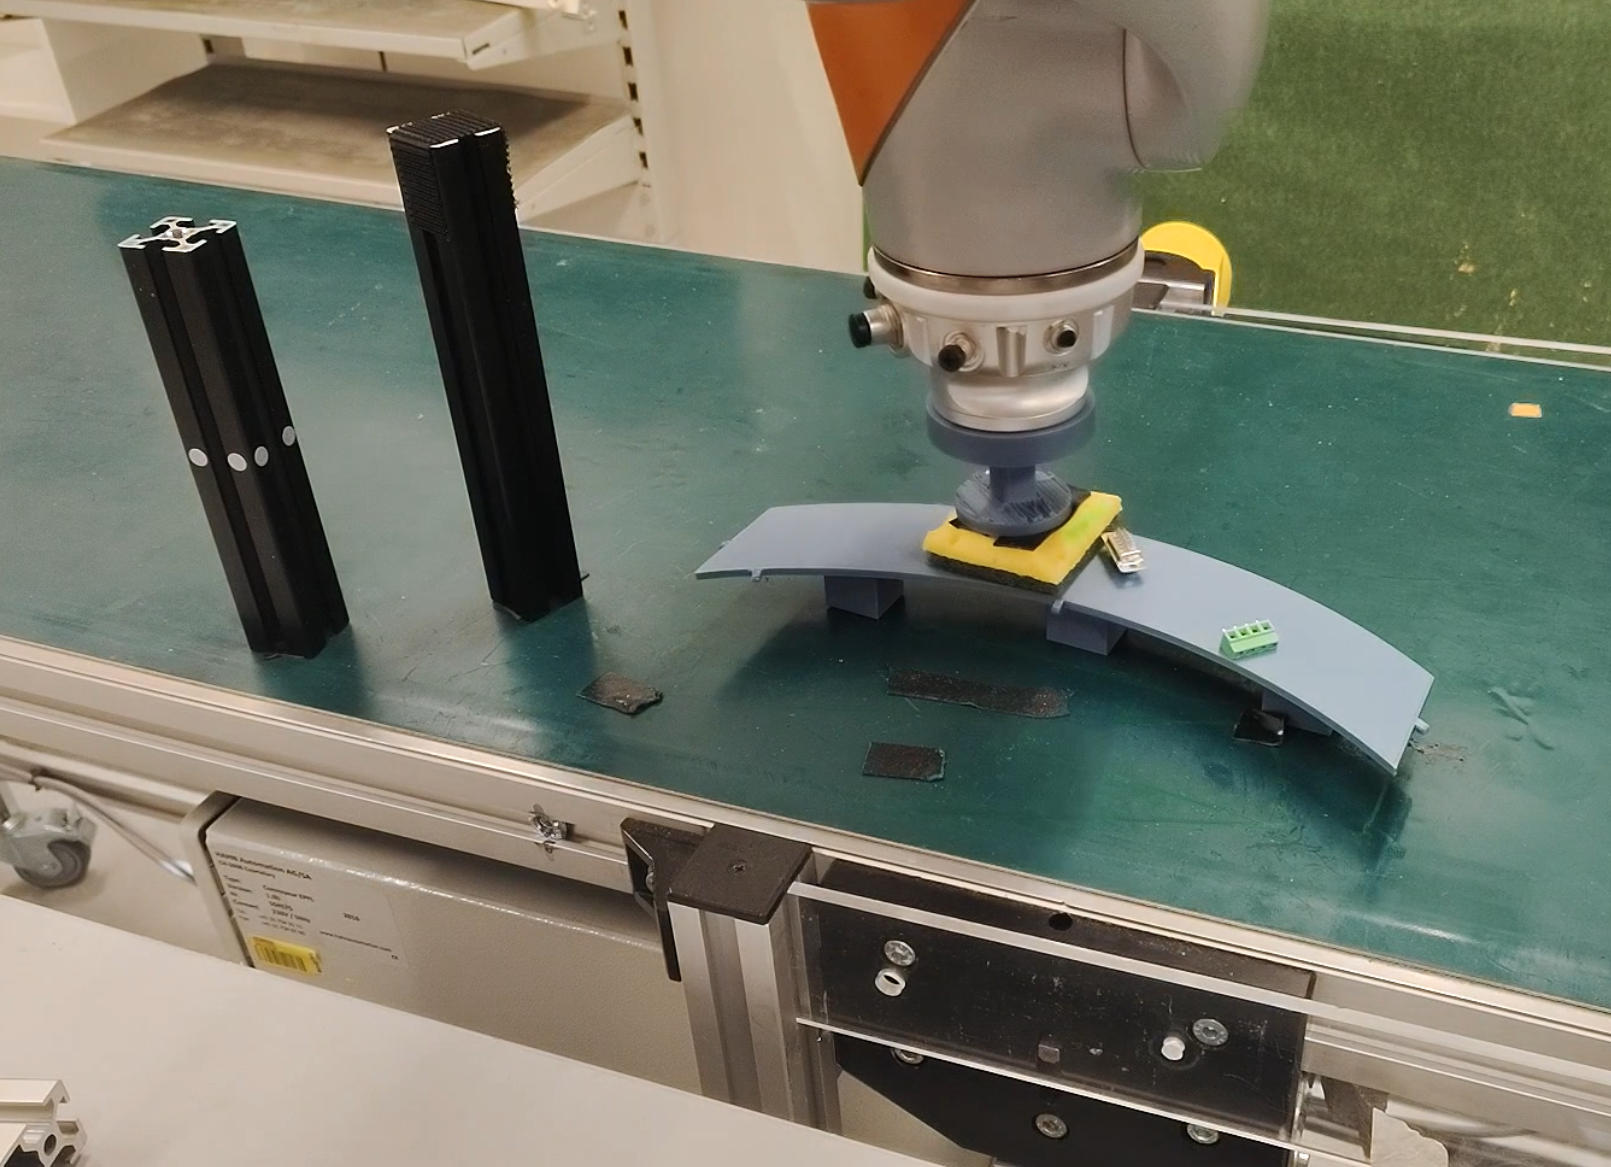
\includegraphics[width=0.98\linewidth]{figs/barclear_transfer.png}
    \caption{Transfer setting with a curved bar and an additional obstacle. The known curved-bar geometry is used to compute the task features, while the learned stage-wise constraints are reused without modification.}
    \label{fig:barclear_transfer}
\end{figure}



\section{Preliminaries and Problem Formulation}

We consider multi-stage tasks whose valid executions are characterized by known stage-independent feasibility requirements and unknown stage-dependent constraints on task features. Let $\mathcal{X}\subseteq\mathbb{R}^{d_x}$ denote the state space, and let $\Phi=\{\phi_j:\mathcal{X}\rightarrow\mathbb{R}\}_{j=1}^{F}$ be a given task-dependent feature bank. For a state $x_t$, the full feature vector is $\phi(x_t)=[\phi_1(x_t),\dots,\phi_F(x_t)]^\top\in\mathbb{R}^{F}$. Before learning, each feature dimension is standardized over the demonstrated data.

A task consists of $K$ ordered stages. Each stage $k$ is associated with a prescribed subgoal $g_k\in\mathcal{X}$ that specifies its endpoint, where $g_K=x_{\mathrm{goal}}$ is the terminal goal. For a trajectory $\tau=\{x_t\}_{t=1}^{T}$, its stage schedule is represented by cutpoints $B=\{b_k\}_{k=0}^{K}$ satisfying $1=b_0<b_1<\cdots<b_K=T+1$. The cutpoints induce the stage intervals $\mathcal{I}_k(B)=\{b_{k-1},\dots,b_k-1\}$. When learning from demonstrations, these cutpoints are unobserved and may differ across trajectories.

The unknown stage-wise constraint model is represented by a mode matrix $\Gamma=[\gamma_{k,j}]\in\{\varnothing,\mathrm{eq},\mathrm{lb},\mathrm{ub}\}^{K\times F}$. Here, $\gamma_{k,j}=\varnothing$ indicates that feature $j$ is unconstrained in stage $k$, while $\mathrm{eq}$, $\mathrm{lb}$, and $\mathrm{ub}$ denote an equality constraint, a lower-bound inequality, and an upper-bound inequality, respectively.

Each feature is assigned a known admissible constraint family. The feature indices are partitioned into an equality-type set $\mathcal{F}_{\mathrm{eq}}$ and an inequality-type set $\mathcal{F}_{\mathrm{ineq}}$. This prior specifies the admissible constraint type when a feature is active, but not whether it is active in a particular stage. For an inequality-type feature, the lower- or upper-bound direction is also unknown. Accordingly, the admissible modes are restricted as
\begin{equation}
\gamma_{k,j}\in
\begin{cases}
\{\varnothing,\mathrm{eq}\}, & j\in\mathcal{F}_{\mathrm{eq}},\\
\{\varnothing,\mathrm{lb},\mathrm{ub}\}, & j\in\mathcal{F}_{\mathrm{ineq}}.
\end{cases}
\label{eq:admissible_constraint_modes}
\end{equation}

For every active stage-feature pair, $\eta_{k,j}\in\mathbb{R}$ denotes its scalar constraint parameter. It specifies the target feature value for an equality constraint and the boundary value for an inequality constraint. The collection of active parameters is denoted by $\mathcal{P}=\{\eta_{k,j}:\gamma_{k,j}\neq\varnothing\}$. The mode and parameter of each stage-feature pair induce the feasible set
\begin{equation}
\mathcal{C}_{k,j}
=
\begin{cases}
\mathcal{X},
& \gamma_{k,j}=\varnothing,\\
\{x\in\mathcal{X}:\phi_j(x)=\eta_{k,j}\},
& \gamma_{k,j}=\mathrm{eq},\\
\{x\in\mathcal{X}:\phi_j(x)\geq\eta_{k,j}\},
& \gamma_{k,j}=\mathrm{lb},\\
\{x\in\mathcal{X}:\phi_j(x)\leq\eta_{k,j}\},
& \gamma_{k,j}=\mathrm{ub}.
\end{cases}
\label{eq:stage_feature_feasible_set}
\end{equation}

Given the stage-wise constraint model $(\Gamma,\mathcal{P})$, a trajectory length $T$, a start state $x_{\mathrm{start}}$, and the ordered subgoals $\{g_k\}_{k=1}^{K}$, a valid task execution is defined as a solution to the following feasibility problem:
\begin{equation}
\begin{aligned}
\text{find}\quad
& \tau=\{x_t\}_{t=1}^{T},\quad B=\{b_k\}_{k=0}^{K} \\
\text{s.t.}\quad
& 1=b_0<b_1<\cdots<b_K=T+1,\\
& x_1=x_{\mathrm{start}},\\
& x_{b_k-1}=g_k,
\qquad k=1,\dots,K,\\
& \tau\in\mathcal{C}_{\mathrm{known}},\\
& x_t\in\bigcap_{j=1}^{F}\mathcal{C}_{k,j},
\qquad
t\in\mathcal{I}_k(B),\quad k=1,\dots,K.
\end{aligned}
\label{eq:stagewise_feasibility_problem}
\end{equation}
Here, $\mathcal{C}_{\mathrm{known}}$ contains known trajectory-level feasibility requirements, such as system dynamics and known collision-avoidance constraints.

We are given a set of feasible demonstrations $\mathcal{D}=\{\tau^{(i)}\}_{i=1}^{N}$, where $\tau^{(i)}=\{x_t^{(i)}\}_{t=1}^{T_i}$. The demonstrations may have different lengths, start states, subgoals, and latent stage schedules, but share the same number and ordering of stages and the same stage-wise constraint model $(\Gamma,\mathcal{P})$. Each demonstration is assumed to satisfy \eqref{eq:stagewise_feasibility_problem} under its true latent schedule.

\begin{definition}[Stage-wise constraint learning from demonstrations]
Given feasible demonstrations $\mathcal{D}$, the number of stages $K$, the feature bank $\Phi$, and the known feature-family sets $\mathcal{F}_{\mathrm{eq}}$ and $\mathcal{F}_{\mathrm{ineq}}$, stage-wise constraint learning aims to recover:
\begin{enumerate}
    \item the shared constraint mode matrix $\Gamma=[\gamma_{k,j}]$, which specifies the active constraint mode of every stage-feature pair;
    \item the active scalar constraint parameters $\mathcal{P}=\{\eta_{k,j}:\gamma_{k,j}\neq\varnothing\}$.
\end{enumerate}
The stage assignments and subgoals are not given, and they will be jointly estimated during learning as auxiliary latent variables.
\end{definition}
